\documentclass[12pt,a4paper]{report}

\usepackage[utf8]{inputenc}
\usepackage[T1]{fontenc}
\usepackage{lmodern}
\usepackage{titlesec} 
\usepackage{graphicx}
\usepackage{microtype}
\usepackage{hyperref} 
\usepackage{amssymb}
\usepackage[frenchb]{babel}
\usepackage{listings}
\usepackage{amsmath}
\usepackage{enumitem}
\usepackage{float} 

\usepackage{pict2e}

\usepackage{listings}	  

\lstdefinestyle{customstyle}{
    basicstyle=\footnotesize,
    breakatwhitespace=false,         
    breaklines=true,                 
    captionpos=b,                    
    keepspaces=true,                                                                                       
    tabsize=4,
    frame=single,
    moredelim=[is][\underbar]{_}{_}
}
\lstset{style=customstyle}

\title{Projet de recherche}
\author{Antoine Forgerou \and Jérémy Bardon \and Nicolas Bourdin}
\date{}
\titleformat{\chapter}[hang]{\bf\huge}{\thechapter}{2pc}{} %Permet de masquer les affichages de "Chapitre" 
\begin{document}
	\renewcommand{\contentsname}{Sommaire}
	\maketitle	

	\tableofcontents	
	\newpage
	
	\setlength{\unitlength}{1cm}

\chapter{Présentation du laboratoire}
Acteur central du développement de l'informatique dans la région des Pays de La Loire, le LINA (Laboratoire d'Informatique de Nantes Atlantique) est un laboratoire de recherche en sciences et technologies du logiciel qui est dirigé par Pierre Cointe. Avec ses 180 membres, ce laboratoire est actuellement situé sur deux sites Nantais : la Lombarderie (Faculté des Sciences et Techniques) et la Chantrerie (Ecole des Mines et Polytech' Nantes).


\section{Les différentes équipes}
Le LINA est composé des équipes suivantes : 
\begin{itemize}
  \item AeLoS : \textbf{A}rchitecture et \textbf{Lo}giciel \textbf{S}ûrs
  \item ASCOLA : \textbf{AS}pect and \textbf{CO}mposition \textbf{LA}nguages
  \item AtlanMod : \textbf{Atlan}tic \textbf{Mod}eling 
  \item COD : \textbf{CO}nnaissances et \textbf{D}écision
  \item ComBi : \textbf{Com}binatoire et \textbf{Bi}oinformatique
  \item DUKe : \textbf{D}ata \textbf{U}ser \textbf{K}nowledg\textbf{e}
  \item GDD : \textbf{G}estion de \textbf{D}onnées \textbf{D}istribuées
  \item GRIM : \textbf{G}estion, \textbf{R}ésumé, \textbf{I}nterrogation, et apprentissage sur les \textbf{M}asses de données
  \item OPTI : Optimisation globale, optimisation multi-objectifs
  \item TALN : \textbf{T}raitement \textbf{A}utomatique du \textbf{L}angage \textbf{N}aturel
  \item TASC : Programmation par contraintes
\end{itemize}

\chapter{L'équipe AeLoS}	

L'équipe AeLoS, dirigé par Christian ATTIOGBE, est une équipe de recherche intégrée au LINA résultant de la fusion de deux anciennes équipes COLOSS et MODAL.

Le projet central de cette équipe s'appuie sur les trois thématiques suivantes :
\begin{itemize}[label=$\circ$]
  \item Architecture : 
  \item Composants logiciels corrects : 
  \item Multiformalisme et analyse multifacette : 
\end{itemize}

\section{Les membres}
Voici la liste des membres actuels de l'équipe AeLoS : \\
\begin{itemize}
  \item Membres permanents :\\
  \begin{itemize}[label=$\circ$]
    \item ANDRE Pascal (MC)
    \item ARDOUREL Gilles (MC)
    \item ATTIOGBE Christian (P)
    \item DELAHAYE Benoit (MC)
    \item JARD Claude (P)
    \item LANOIX Arnaud (MC)
    \item MOTTU Jean-Marie (MC)
    \item OUSSALAH CHABANE Mourad (P)
    \item TAMZALIT Dalila (MC)
    \item VAILLY Alain (MC)\\
  \end{itemize}
  
  \item Membres non permanents :\\
  \begin{itemize}[label=$\circ$]
    \item AOUADHI Mohamed Amine (D)
    \item DAVID Nicolas (D)
    \item GASMALLAH Noureddine (D)
    \item HASSAN Adel (D)
    \item PEPIN Jonathan (D)
    \item PERRIN Matthieu (D)
    \item SFERRUZZA David (D)\\
  \end{itemize} 
\end{itemize}

MC : Maître de conférence, P : Profeseur, D : Doctorant\\


\chapter{Présentation du sujet}
\section{Problématique}

\paragraph*{Contexte} : Approches formelle des systèmes embarqués communiquants.\\

La construction rigoureuse d'un logiciel se fait à partir de son modèle. Pour des logiciels complexes (par exemple ceux
qui ont de nombreux composants différents -- hétérogènes-- et qui communiquent), on a affaire à plusieurs modèles
(hétérogènes aussi) qui doivent intérargir de façon cohérente, pour garantir l'interopérabilité sémantique entre les
modèles puis les composants logiciels. Le domaine des systèmes embarqués (et aussi des objets connectés) regorge
d'exemples.\\

\paragraph*{Description du travail} : Etudier l'interopérabilité entre des modèles de composants (logiciels ou non).\\
En nous appuyant dans un premier temps sur des modèles à base d'automates à états, il s'agit dans le cadre du stage
d'initiation à la recherche, de contribuer à la conception et au développement d'outils passerelle entre modèles.\\\\

Nous travaillons sur plusieurs aspects :\\
\begin{itemize}
  \item Lorsque cela est possible, en fonction de la sémantique des modèles, un modèle donné est encodé par un autre
modèle choisi mais qui est sémantiquement équivalent.
  \item Lorsque cela est possible, en fonction de la sémantique des modèles, un modèle peut interagir avec un autre avec
des contrats (de type Assume/Guarantee)
  \item Plug'N'Check (analyse systématique de modèles/composants)
  \item etc
\end{itemize}

\section{Solutions proposées par l'équipe AeLoS}
Pour répondre à la problématique, l'équipe AeLoS nous a proposé 3 façons de 
faire tout en nous laissant la liberté d'en proposer d'autres.
\\\\
Dans le but de simplifier les exemples, nous avons fait le choix de représenter 
les modèles comme des formes géométriques que l'on essayerai d'emboiter.
\\\\
La première solution consiste à adapter un des modèles au deuxième quand cela 
est possible. On peut prendre l'exemple du théorème de Kleene qui assure qu'un 
automate à états finis peut être écrit sous la forme d'une expression 
rationnelle et vice et versa.

\begin{figure}[h]
	\centering
	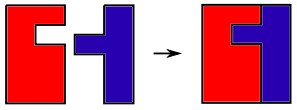
\includegraphics[scale=1]{ressources/solution1.png}
	\caption{Solution 1 - Adaptation d'un modèle}
\end{figure}
\newpage
L'approche qui parait la plus évidente mais qui peut se révéler complexe 
consiste à intégrer un troisième modèle dans le système. Ce dernier va alors 
jouer le rôle de passerelle entre les deux modèles que l'on veut faire 
communiquer.

\begin{figure}[h]
	\centering
	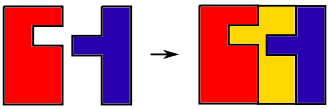
\includegraphics[scale=1]{ressources/solution2.png}
	\caption{Solution 2 - Interface entre les modèles}
\end{figure}

Plug'N'Check est le nom de la troisième solution que l'équipe nous a soumise. 
Le principe est de faire interagir les modèles ensemble puis d'effectuer des 
vérifications pour déterminer si les modèles peuvent communiquer à 100\%, 
en partie ou pas du tout.

\begin{figure}[h]
	\centering
	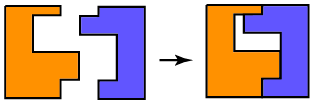
\includegraphics[scale=1]{ressources/solution3.png}
	\caption{Solution 3 - Plug'N'Check}
\end{figure}

Dans le cadre de notre stage d'initiation à la recherche, nous nous sommes 
orientés vers la première solution. Nous avons donc entrepris de transformer 
n'importe quel modèle dans un language commun afin de permettre de les 
interfacer.

\newpage
\section{UPPAAL : un outil de modelisation des automates}
UPPAAL est un environnement intégré d'outils pour la modélisation , la validation et la vérification des systèmes temps réel modélisés comme des réseaux d' automates.
Uppaal se compose de trois parties principales: 
\begin{itemize}[label=$\circ$]
  \item{ un langage de description}
  \item{ un simulateur}
  \item{ un vérificateur de modèle}
\end{itemize} 

  Le langage de description est un langage de commande non-déterministe avec des types de données (par exemple des entiers , des tableaux, etc. ) . Il ce sert de la modélisation ou du langage de conception pour décrire le comportement du système grâce à des réseaux d'automates étendus avec des variables d' horloge et des données .\\ 

  Le simulateur est un outil de validation qui permet l'examen de possibles exécutions d'un système au début de la conception( ou la modélisation ) et fournit un moyen peu coûteux de détection de défaut avant la vérification par le vérificateur de modèle qui couvre l'ensemble des comportement dynamique du système.\\

  Le modèle orthographique peut vérifier les propriétés invariantes et l'accessibilité en explorant l'espace et l'état d'un système, c'est à dire l'analyse de l'accessibilité en termes d'états symboliques représentés par des contraintes .

\section{Le format DOT}

  Le langage DOT est un langage de description de graphe dans un format texte. C'est une manière simple de décrire des graphiques que les humains et les programmes informatiques peuvent utiliser. Les graphes DOT sont généralement des fichiers avec pour extension un .gv (ou .dot ).\\

  La syntaxe DOT peut aussi bien décrire des graphes non-orientés que des graphes orientés, comme des automates finis.
  Il est possible de placer des labels sur les transistions pour par exemple leurs donner un nom ou une explication. Le language possède aussi des attributs permettant une description graphique plus poussée, par exemple choisir la couleur d'un noeud ou de dessiner une transition en pointillé.

\subsection{Graphe non-orienté}

\begin{lstlisting}
graph monGraphe {
    a -- b -- c;
    b -- d;
}
\end{lstlisting}

  \textit{Resultat : }

\begin{figure}[!h]
  \centering
  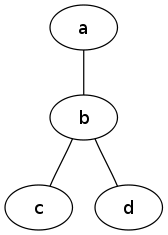
\includegraphics[scale=0.3]{ressources/grapheNO.png}
\end{figure}

\subsection{Graphe orienté}

\begin{lstlisting}
graph monGraphe {
    a -> b -> c;
    b -> d;
}
\end{lstlisting}

\begin{figure}[!h]
  \centering
  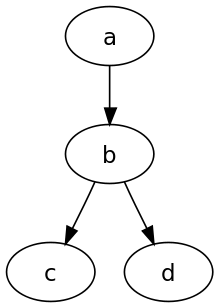
\includegraphics[scale=0.3]{ressources/grapheO.png}
\end{figure}


\end{document}
